\documentclass{beamer}

\usepackage{Haust2016glærur}

\title{Stærðfræðimynstur í tölvunarfræði}
\subtitle{Vika 9, seinni fyrirlestur}

\begin{document}

\begin{frame}
\titlepage
\end{frame}


\section{Inngangur}

\begin{frame}{Í síðasta tíma}
\begin{itemize}
 \item Inngangur að venslum
\end{itemize}
\end{frame}

\begin{frame}[fragile]{Leiðrétting}

\begin{tcolorbox}[title={\color{red}Gegnvirk} vensl]
Vensl $R$ á mengi $A$ eru {\color{red}gegnvirk} (e. \emph{transitive}) ef, hvenær sem $(a, b) \in R$ og $(b, c) \in R$, þá sé $(a, c) \in R$, fyrir öll $a, b, c \in A$. Þ.e.a.s. vensl $R$ á mengi $A$ eru {\color{red}gegnvirk} þegar $\forall a\forall b\forall c(((a, b) \in R \land (b, c) \in R) \to (a, c) \in R)$
\end{tcolorbox}
\begin{columns}
\column{0.5\textwidth}
Gegnvirk vensl:
\begin{align*}
R_1 &= \{(a, b)|a \leq b\}\\
R_2 &= \{(a, b)|a > b\}\\
R_3 &= \{(a, b)|a = b \text{ eða } a = -b\}\\
R_4 &= \{(a, b)|a = b\}\\
\end{align*}
\column{0.5\textwidth}
Ekki gegnvirk vensl:
\begin{align*}
R_5 &= \{(a, b)|a = b+1\}\\
R_6 &= \{(a, b)|a+b \leq 3\}\\
\end{align*}
\end{columns}
\end{frame}

\section{Miðmisserispróf}

\begin{frame}{Miðmisserispróf}
\begin{columns}
\column{0.3\textwidth}
\begin{itemize}
 \item 144 af 225 tóku prófið
 \item Meðaleinkunn var 6.20
 \item Algengasta (námundaða) einkunn var 7.5
 \item Þrír nemendur með 10.0 ónámundað
\end{itemize}
\column{0.7\textwidth}
\begin{center}
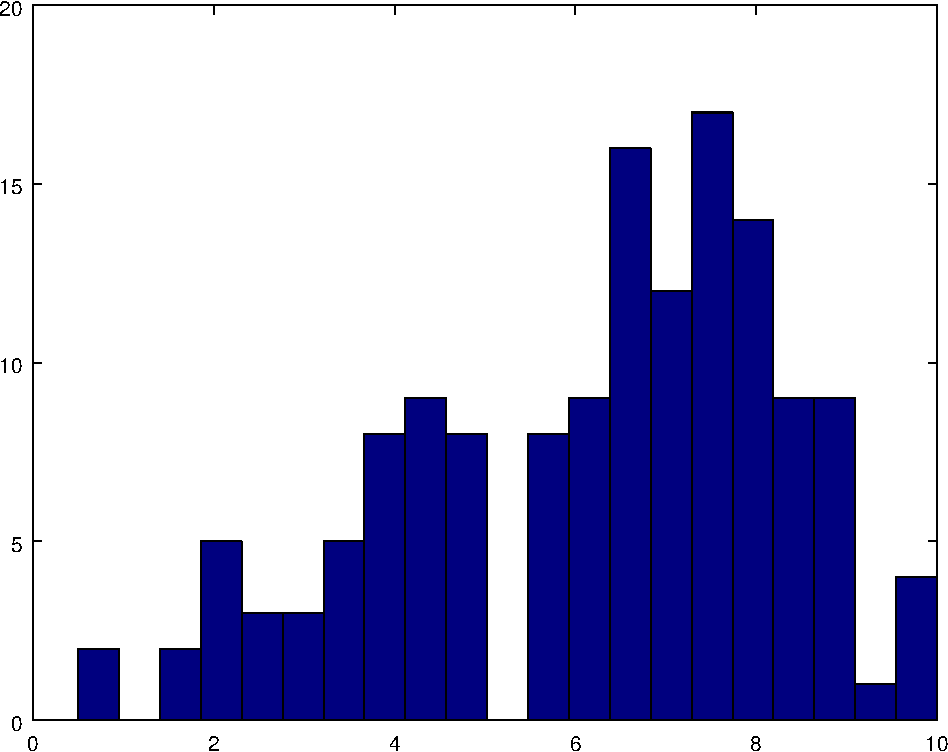
\includegraphics[width=\linewidth]{midmisserisprof2016dreifing}
\end{center}
\end{columns}
\end{frame}


\begin{frame}{Dreifing eftir dæmum}
\begin{columns}
\column{0.3\textwidth}
Dæmi númer 1 til 7 frá vinstri til hægri. 5 stiga dæmi sköluð upp í 10 punkta til samanburðar.
\column{0.7\textwidth}
\begin{center}
\includegraphics[width=\linewidth]{midmisserisprof2016daemadreifing}
\end{center}
\end{columns}
\end{frame}

\section{N-undarvensl og gagnagrunnar}

\begin{frame}{$n$-undarvensl}
\begin{itemize}
 \item Í síðasta tíma skoðuðum við tvíundarvensl (vensl á tvö mengi) og vensl á mengi (eitt mengi)
 \item Oft koma upp vensl á milli tveggja eða fleiri mengja
 \item Köllum vensl á milli $n$ mengja $n$-undarvensl (e. \emph{n-ary relations})
\end{itemize}
\end{frame}

\begin{frame}{Skilgreining}
\begin{tcolorbox}[title=n-undarvensl]
Látum $A_1, A_2, \ldots, A_n$ vera mengi. $n$-undarvensl á mengin er hlutmengi $A_1 \times A_2 \times \ldots \times A_n$. Mengin $A_1, A_2, \ldots, A_n$ eru þá óðöl (e. \emph{domains}) venslanna og talan $n$ er stig (e. \emph{degree}) þeirra. Stak í $n$-undarvenslum er $n$-und (e. \emph{$n$-tuple}).
\end{tcolorbox}
\end{frame}

\begin{frame}{Dæmi}
Látum $R$ vera vensl sem mynda hlutmengi í $N \times N \times N$ á þann hátt að hver röðuð 3-und $(a, b, c) \in R$ hefur eiginleikann $a < b < c$. Þá er $(1, 2, 3) \in R$ en $(2, 4, 3) \notin R$. Stig þrenndarinnar er 3. Óðöl þrenndarinnar eru öll mengi náttúrulegu talnanna.
\end{frame}

\begin{frame}[fragile]{Dæmi}
Við getum myndað vensl á mengin ``nafn'', ``auðkenni'', ``námsbraut'' og ``ferileinkunn''. 4-undir sem gætu tilheyrt þessum venslum eru:

\begin{verbatim}
(Ackermann,  231455, Computer Science, 3.88)
(Adams,      888323, Physics,          3.45)
(Chou,       102147, Computer Science, 3.49)
(Goodfriend, 453876, Mathematics,      3.45)
(Rao,        678543, Mathematics,      3.90)
(Stevens,    786576, Psychology,       2.99)
\end{verbatim}
Við getum séð fyrir okkur að þessi vensl séu hluti af gagnagrunni (e. \emph{database}) þar sem hvert óðal skilgreinir eigind (e. \emph{attribute}). 
\end{frame}

\begin{frame}[fragile]{Dæmi}
\begin{columns}
\column{0.4\textwidth}
\begin{itemize}
 \item Við getum sett fram venslin á fyrri glæru með því að nota töflu
 \item Getum þá notað annað orðalag:
 \begin{itemize}
  \item Eigind: Svið (e. \emph{field}) eða ``dálkur''
  \item $n$-und: Færsla (e. \emph{record}) eða ``lína''
 \end{itemize}
\end{itemize}
\column{0.6\textwidth}
\begin{center}
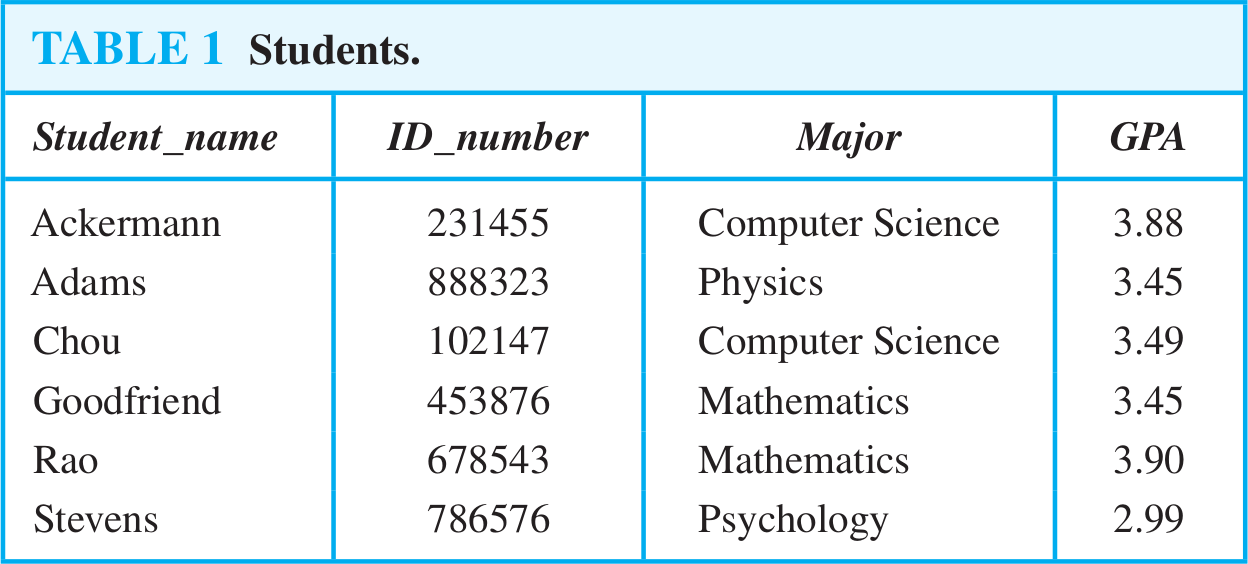
\includegraphics[width=\linewidth]{relation-table}
\end{center}
\end{columns}
\end{frame}

\begin{frame}{Hugtök úr gagnasafnsfræði}
\begin{itemize}
 \item ``Superkey'' - samsetning á eigindum sem auðkenna hverja $n$-und venslanna einkvæmt
 \begin{itemize}
  \item Þ.e.a.s. einhver dálkur eða dálkar sem duga sem auðkenni fyrir hverja línu
 \end{itemize}
 \item Superkey af lágmarksstærð er ``Candidate Key''
 \begin{itemize}
  \item ``Primary Key'' er sá lykill sem valinn hefur verið sá mest viðeigandi af öllum Candidate Keys
  \begin{itemize}
   \item Viljum ekki að Primary Key sé háður gögnunum, oft er sérstakur dálkur búinn til
  \end{itemize}
 \end{itemize}
 \item ``Intension of a relation'' - fastir eiginleikar vensla
 \item ``Extension of a relation'' - þær $n$-undir sem birtast í venslunum á einhverjum tímapunkti
\end{itemize}
\end{frame}

\section{Venslaaðgerðir}

\begin{frame}{Val}
Við getum skilgreint aðgerðir fyrir $n$-undarvensl. Slíkar aðgerðir gætu unnið með gögn í gagnagrunnum.

\vspace{0.5cm}
Skilgreinum valvirkjann, sem velur $n$-undir úr venslum: 
\begin{tcolorbox}[title=Valvirkinn]
Látum $R$ vera $n$-undarvensl og $C$ vera skilyrði sem stök í $R$ geta uppfyllt. Þá varpar valvirkinn $s_C$ (e. \emph{selection operator}) venslunum $R$ yfir í vensl allra $n$-unda úr $R$ sem uppfylla skilyrðin $C$.
\end{tcolorbox}
\end{frame}

\begin{frame}{Dæmi}
\begin{columns}
\column{0.5\textwidth}
Notum valvirkjann $s_{C_{CS}}$, þar sem skilyrðið $C_{CS}$ er skilyrðið ``námsbrautin er tölvunarfræði''.
\vspace{0.5cm}

Notum þennan virkja á venslin hér til hliðar. Fáum önnur vensl sem innihalda $n$-undir eitt og þrjú (talið að ofan).
\column{0.5\textwidth}
\begin{center}
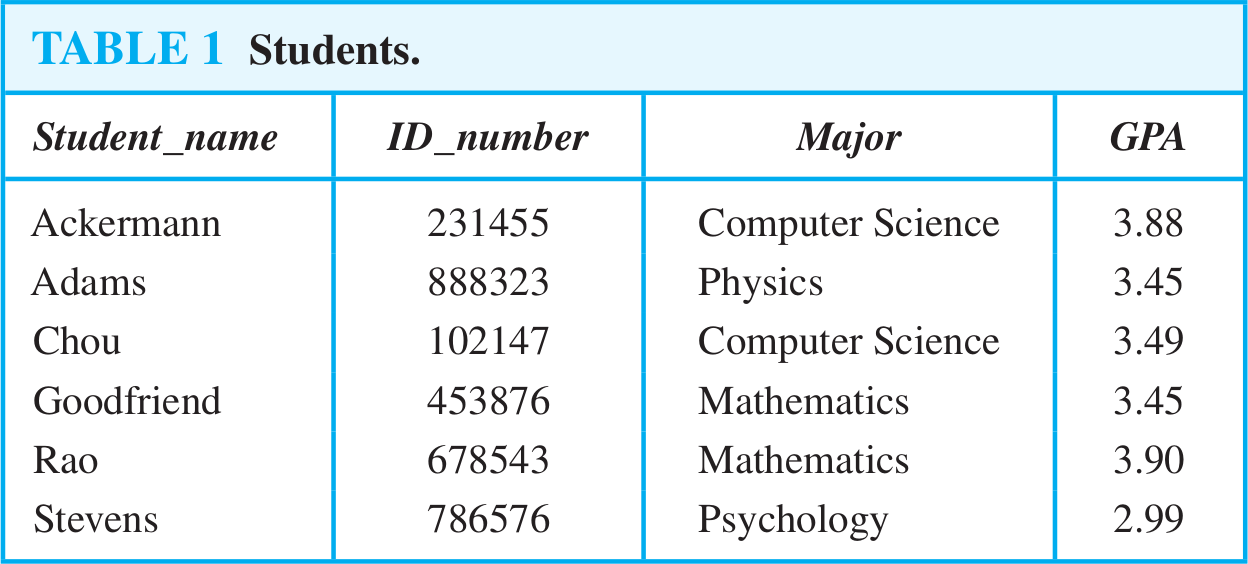
\includegraphics[width=\linewidth]{relation-table}
\end{center}
\end{columns}
\end{frame}

\begin{frame}{Dálkval}
Skilgreinum dálkvalsvirkja, sem velur eigindi úr venslum:

\begin{tcolorbox}[title=Dálkval]
Dálkvalsvirkinn $P_{i_1, i_2, \ldots, i_m}$ þar sem $i_1 < i_2 < \ldots < i_m$ varpar $n$-undinni $(a_1, a_2, \ldots, a_n)$ yfir $m$-undina $(a_{i_1}, a_{i_2}, \ldots, a_{i_m})$, þar sem $m \leq n$.
\end{tcolorbox}
Sem sagt, $P_{i_1, i_2, \ldots, i_m}$ eyðir $n-m$ eigindum úr hverjum $n$-undum sem tilheyra venslunum sem hann er notaður á.
\end{frame}

\begin{frame}{Dæmi}
\begin{columns}
\column{0.4\textwidth}
Notum dálkvalvirkjann $P_{1,4}$ á venslin hér til hliðar.

\vspace{0.5cm}
Fáum vensl sem innihalda tvenndir sem innihalda nafn sem fyrra stak og ferileinkunn sem seinna stak.

\vspace{0.5cm}
Athugum - vensl eru mengi, svo fjöldi aðskilinna staka getur fækkað við dálkval.
\column{0.6\textwidth}
\begin{center}
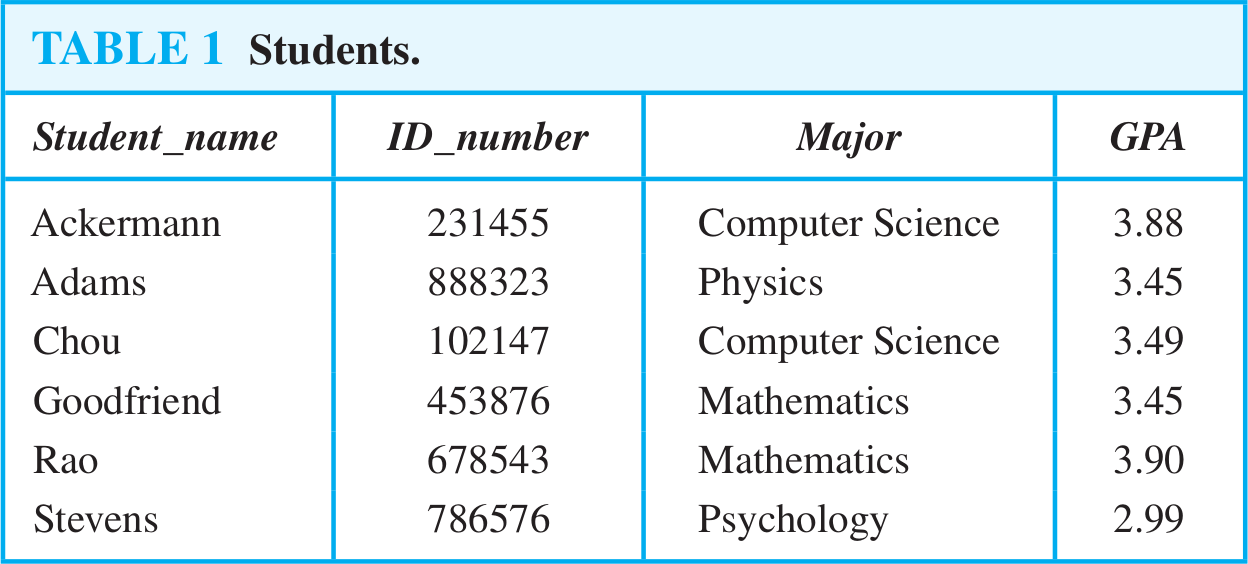
\includegraphics[width=\linewidth]{relation-table}
\end{center}
\end{columns}
\end{frame}

\begin{frame}{Tenging}
Hægt er að tengja tvö vensl saman með því að nota sameiginleg eigindi þeirra.

\begin{tcolorbox}[title=Tenging]
Látum $R$ vera $m$-ta stigs vensl og $S$ vera $n$-ta stigs vensl. Tengingin $J_p(R,S)$, þar sem $p\leq m$ og $p \leq n$, er vensl af stigi $m+n-p$ sem inniheldur allar $(m+n-p)$-undir $(a_1, a_2, \ldots, a_{m-p}, c_1, c_2, \ldots, c_p, b_1, b_2, \ldots b_{n-p})$ þar sem $m$-undin $(a_1 , a_2 , \ldots , a_{m-p} , c_1 , c_2 , \ldots , c_p )$ er í $R$ og $n$-undin $(c_1 , c_2 , \ldots , c_p , b_1 , b_2 , \ldots , b_{n-p} )$ tilheyrir $S$.
\end{tcolorbox}

\end{frame}

\begin{frame}{Dæmi}
Notum $J_2$ á eftirfarandi vensl:
\begin{center}
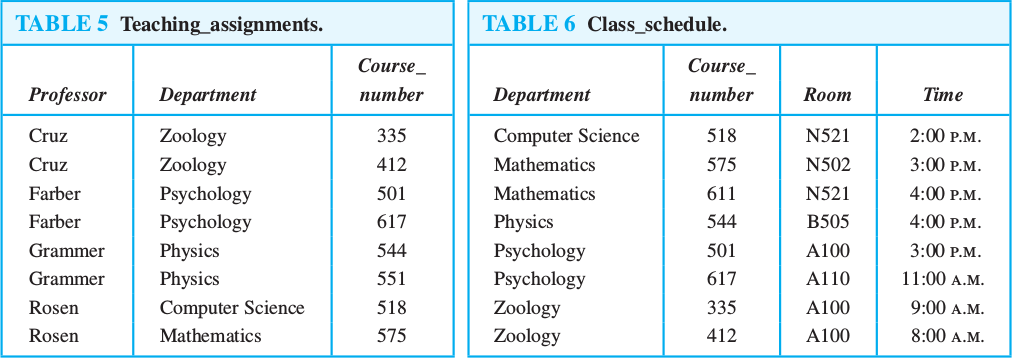
\includegraphics[width=\textwidth]{relation-join-tables}
\end{center}
\end{frame}
\begin{frame}{Niðurstaða}
\begin{center}
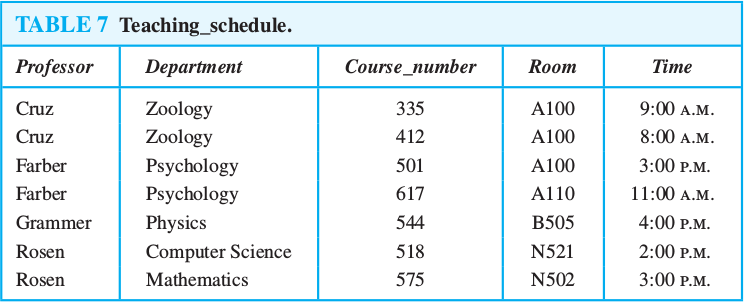
\includegraphics[width=\textwidth]{relation-join-table-result}
\end{center}
\end{frame}

\begin{frame}[fragile]{SQL}
\begin{columns}
\column{0.4\textwidth}
Fyrirspurnarmálið SQL er hægt að nota til að eiga samskipti við gagnagrunna.
\vspace{0.5cm}
\begin{minted}{sql}
SELECT Departure_time
FROM Flights
WHERE Destination='Detroit';
\end{minted}

\column{0.6\textwidth}
\begin{center}
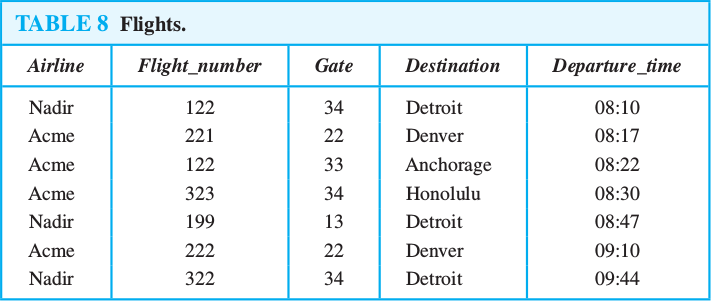
\includegraphics[width=\linewidth]{flight-table}
\vspace{1cm}
\end{center}
\end{columns}
\end{frame}

\begin{frame}{Dæmi}
Lítum á join í SQL: \url{http://sqlfiddle.com/\#!9/14848/1}
\end{frame}

\section{Framsetning vensla með fylkjum}

\begin{frame}{Vensl og fylki}
\begin{itemize}
 \item Líkt og við settum áður fram tvíundarvensl með töflu, þá getum við sett tvíundarvensl með því að nota fylki
 \item Látum venslin $R$ vera tvíundarvensl á mengin $A = \{a_1, a_2, \ldots, a_m \}$ og $B = \{b_1, b_2, \ldots, b_n\}$
 \item Þá getum við skilgreint tvíundarfylki þar sem stökin eru:
\end{itemize}
\[
 m_{ij} = \left\{
\begin{matrix}
1 \text{ ef } (a_i, b_j) \in R\\
0 \text{ ef } (a_i, b_j) \notin R\\
\end{matrix}\right.
\]
\end{frame}

\begin{frame}{Dæmi}
Látum $A= \{1, 2, 3\}$ og $B = \{1, 2\}$ og $R$ vera vensl frá $A$ til $B$ þar sem $a > b$, $a \in A$ og $b \in B$. Hvert er fylkið sem táknar $R$?\\
\pause
Fáum að $R= \{(2, 1), (3, 1), (3, 2)\}$. Setjum ása á viðeigandi staði í $M$, fáum 
\[
 M_R =
\begin{bmatrix}
0 & 0\\
1 & 0\\
1 & 1\\
\end{bmatrix}
\]
\end{frame}

\begin{frame}{Athuganir um fylkjaframsetningu}
\begin{columns}
\column{0.6\textwidth}
\begin{itemize}
 \item Vensl á mengi (eitt mengi) eru með fylkjaframsetningu sem er ferningsfylki
 \item Vensl $R$ á mengi $A$ eru sjálfhverf (e. \emph{reflexive}) ef $(a, a) \in R$ þegar $a \in A$.
 \item Þá eru vensl sjálfhverf þá og því aðeins að öll stök á aðalhornalínu fylkjaframsetningar þess séu 1
\end{itemize}
\column{0.4\textwidth}
\[
\begin{bmatrix}
1&&&&\\
&1&&&\\
&&\ddots&&\\
&&&1&\\
&&&&1\\
\end{bmatrix}
\]
\end{columns}
\end{frame}

\begin{frame}{Athuganir um fylkjaframsetningu}
\begin{columns}
\column{0.7\textwidth}
\begin{itemize}
 \item $R$ eru samhverf vensl á $A$ ef $(a,b) \in R \to (b, a) \in R$ fyrir öll $a, b \in A$
 \begin{itemize}
  \item Þá er $m_{ij} = m_{ji}$ í fylkjaframsetningunni
 \end{itemize}
 \item $R$ eru andsamhverf vensl á mengi $A$ ef $(a, b) \in R \land (b, a) \in R \to (a = b)$ fyrir öll $a, b \in A$
 \begin{itemize}
  \item Þá er a.m.k. annað af $m_{ij}$ og $m_{ji}$ núll þegar $i\neq j$ 
 \end{itemize}

\end{itemize}
\column{0.3\textwidth}
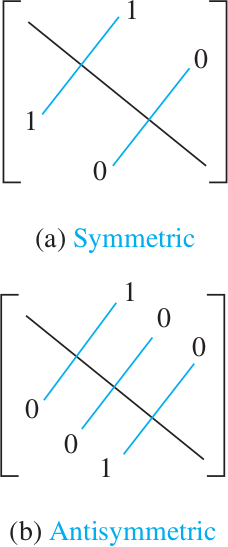
\includegraphics[width=\linewidth]{symmetric-antisymmetric-matrix}
\end{columns}
\end{frame}

\section{Net}

\begin{frame}{Stefnt net}
Skilgreinum í snarhasti hugmynd um \emph{stefnt net}.
\begin{tcolorbox}[title=Stefnt net]
Stefnt net (e. \emph{directed graph}) samanstendur af mengi $V$ af hnútum (e. \emph{vertices} eða \emph{nodes}) og mengi $E$ af röðuðum pörum af hnútum í $V$ sem nefnast stefndir leggir (e. \emph{directed edges}). Í leggnum $(a, b)$ er fyrri hnúturinn upphafshnútur (e. \emph{initial vertex}) og seinni hnúturinn lokahnútur (e. \emph{terminal vertex}).
\end{tcolorbox}
\end{frame}

\begin{frame}{Stefnt net}
Stefnd net eru oftast sett fram á þann hátt að punktar eða hringir tákni hnúta og örvar tákni stefndu leggina.

\begin{center}
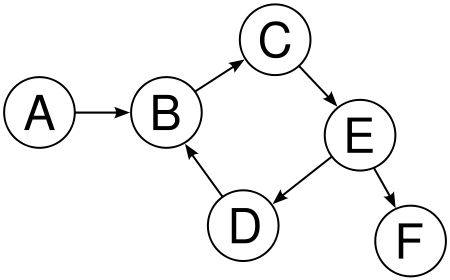
\includegraphics[width=0.6\textwidth]{directed-graph}
\end{center}

\end{frame}

\section{Netaframsetning á venslum}

\begin{frame}{Netaframsetning á venslum}
\begin{itemize}
 \item Við getum sett vensl $R$ á mengið $A$ fram með því að tákna stök $A$ sem hnúta og hvert raðað par $(a, b)$ í $R$ sem stefndan legg
 \item Stefndi leggurinn $(a, a)$ er táknaður með lykkju (e. \emph{loop}) á hnútnum $a$
\end{itemize}
\end{frame}

\begin{frame}{Dæmi}
\begin{columns}
\column{0.5\textwidth}
Venslin
\[
 R = \{(1, 3), (1, 4), (2, 1), (2, 2), (2, 3),
\]
\[
 (3, 1), (3, 3), (4, 1), (4, 3)\}
\]

á mengið $\{1, 2, 3, 4\}$ má tákna með stefnda netinu hér til hægri.
\column{0.5\textwidth}
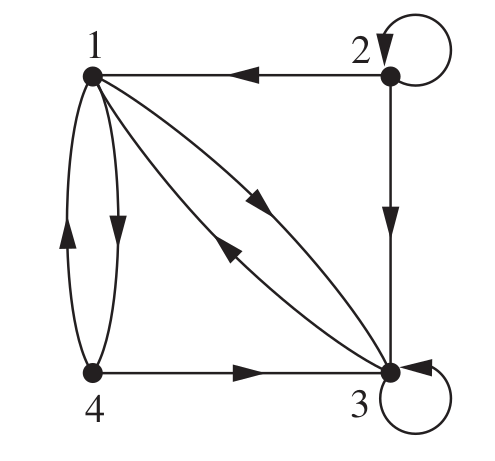
\includegraphics[width=\linewidth]{relational-graph}
\end{columns}
\end{frame}

\begin{frame}{Athuganir um netaframsetningu}
\begin{itemize}
 \item Vensl eru sjálfhverf þá og því aðeins að netaframsetning þeirra hafi lykkju á hverjum hnút
 \item Vensl eru samhverf þá og því aðeins að fyrir hvern stefndan legg $(a,b)$ sé líka til stefndur leggur $(b, a)$
 \begin{itemize}
  \item Milli sömu hnúta, en í gagnstæðar áttir
 \end{itemize}
 \item Vensl eru andsamhverf þá og því aðeins að á milli hverra tveggja hnúta sé aldrei leggur í báðar áttir
\end{itemize}

\end{frame}



\begin{frame}{Næst}
10. kafli, eins langt og við komumst.
\end{frame}


\end{document}
